% \documentclass[]{article}
% \documentclass[onecolumn]{IEEEtran}
% onecolumn for readability
\documentclass[]{IEEEtran}

% -----------------------------------------------------
% Preamble
% -----------------------------------------------------
% Math Packages
\usepackage{physics}
\usepackage{amsmath, amssymb, empheq}
\usepackage{thmtools}
% \usepackage[per-mode=symbol]{siunitx}

% Format Packages/Settings
\usepackage{todonotes}
\usepackage{xcolor}
\usepackage[]{hyperref}
\renewcommand{\figureautorefname}{Fig.}
% \usepackage[inline, shortlabels]{enumitem}
\usepackage{paralist}
\usepackage{cite}
\usepackage{graphicx}


% Theorems
\newtheorem{definition}{Definition}
\newtheorem{theorem}{Theorem}
\newtheorem{lemma}{Lemma}
\newtheorem{corollary}{Corollary}
\newtheorem{remark}{Remark}
\newtheorem{system}{System}

% % Custom Commands
% \newcommand{\R}{\mathbb{R}}
% \newcommand{\N}{\mathbb{N}}
% \newcommand{\st}{ \ | \ }

% \newcommand{\E}{\mathcal{E}}
% \newcommand{\Ebar}{\bar{\mathcal{E}}}
% \newcommand{\X}{\mathcal{X}}
% \newcommand{\Xbar}{\bar{\mathcal{X}}}
% % \newcommand{\U}{\mathcal{U}}
% % \newcommand{\Ubar}{\bar{\mathcal{U}}}
% \newcommand{\F}{\mathcal{F}}


%% Title and stuff
\title{
    Unnamed MPC Project Report
}
\author{Jonas Wagner} % assuming Jonas and Justin... add Tanner?


% -----------------------------------------------------
% Begin Document
% -----------------------------------------------------
\begin{document}

% -----------------------------------------------------
% Title and Abstract
% -----------------------------------------------------
\maketitle
\begin{abstract}
    Insert Abstract
\end{abstract}




% -----------------------------------------------------
% Introduction
% -----------------------------------------------------
\section{Introduction}

\todo{Copy stuff from Proposal}


% -----------------------------------------------------
% Problem Definition
% -----------------------------------------------------
\section{Problem Definition}
\label{sec:pblm_def}



% Path Planning
\subsection{Path Planning}
\label{subsec:pathPlanning}

The objective is to create high-fidelity MPC controller to produce an optimal trajectory to reach a waypoint given the occupancy map of the environment.
This controller will then be used to generate training data for a neural network which will be able to perform an approximation of this controller in real-time.

From the perception stack, the current vehicle states (local and global) will be known to some uncertainty and the surrounding environment will be processed into a predicted occupancy map.
This occupancy map will be assumed to already have weights corresponding to where it is safe/ideal for the vehicle to be in the future.

\todo{add specific math symbols for all these things}




% Model Definition
\subsection{Model Definition}
\label{subsec:mdl_def}
Hail-Bopp will be modeled as a standard 4-wheel ackerman vehicle.
The initial model will be based on the 3-dof bicycle model as derived in \cite{casanova_thesis} and \cite{vehcileDynamics_chapter2a}.


TO DO: 
provide the elaboration of the model...

(so many options... likely assume the local dynamics as just a function of $u$ and $\delta$ and put restrictions on them changing quick?...)


\begin{figure}[h]
    \centering
    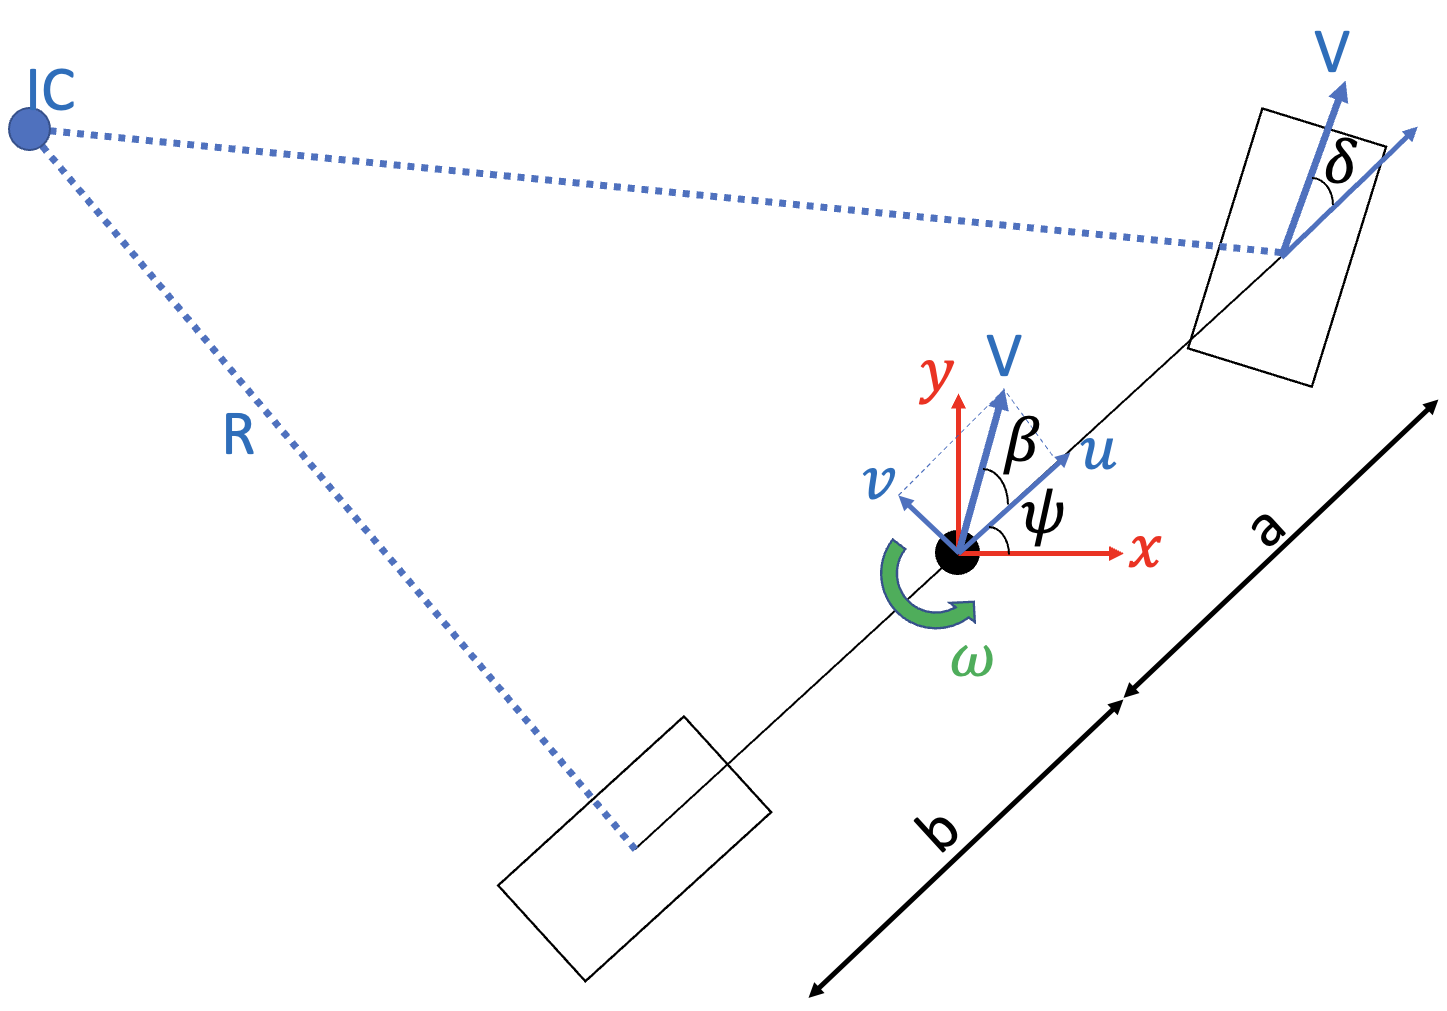
\includegraphics[width=\columnwidth]{figs/BicycleModel.png}
    \caption{}
    \label{fig:bikeModel_diagram}
\end{figure}

Simple non-linear kinematics model equations:
\begin{equation}
    \begin{cases}
        \dot{x} = V \cos(\psi + \beta)\\
        \dot{y} = V \sin(\psi + \beta)\\
        \dot{\psi} = \cfrac{V \cos(\beta)}{l_f + l_r} \qty(tan(\delta_f) - tan(\delta_r))\\
        \dot{theta} = \psi
    \end{cases}
\end{equation}
where
\begin{equation}
    \beta = \tan^-1\qty(\cfrac{l_f \tan(\delta_r) + l_r tan(\delta_f)}{l_f + l_r})
\end{equation}







% -----------------------------------------------------
% Problem Solution
% -----------------------------------------------------
\section{Problem Solution}
\label{sec:pblm_soln}
The MPC Controller for path planning is formulated with the current state and model update equations as hard constraints, an objective to minimize the time and distance to reach the future waypoint, and introducing the occupancy map as soft-constraints within the objective function.

% Model Constraints
\subsection{Model Constraints}



% Cost Function
\subsection{Cost Function}

The primary cost function will be linear from the system state as derived the cost map as the sum of the region that the vehicle would occupy.

Additionally, an objective will be included that describes the foward progression 





% Obstical/Robust constraints
\subsection{Obstical/Robust Constraints}



% % MPC Controller Formulation
% \subsection{MPC Controller Formulation}








% -----------------------------------------------------
% Simulation and Results
% -----------------------------------------------------
\section{Simulation and Results}
\label{sec:sim_and_results}












% -----------------------------------------------------
% Conclusion
% -----------------------------------------------------
\section{Conclusion}
TODO:
add something here...

\cite{MPC_PathTracking} % just to test



% -----------------------------------------------------
% References
% -----------------------------------------------------
\bibliography{refs}{} 
\bibliographystyle{IEEEtran}




\end{document}
